% =====================================================================
% TmFeO3 2DCS — PRL main text
% Condensed from tmfeo3_foundation.tex (34pp working note)
% =====================================================================
\documentclass[aps,prl,twocolumn,superscriptaddress,longbibliography]{revtex4-2}

\usepackage{amsmath,amssymb,bm}
\usepackage{graphicx}
\usepackage{xcolor}
\usepackage{hyperref}
\hypersetup{colorlinks=true,linkcolor=blue,citecolor=blue,urlcolor=blue}

\newcommand{\Fe}{\mathrm{Fe}}
\newcommand{\Tm}{\mathrm{Tm}}
\newcommand{\ket}[1]{|#1\rangle}
\newcommand{\bra}[1]{\langle #1|}
\newcommand{\ve}[1]{\boldsymbol{#1}}
\newcommand{\qafm}{q_{\rm AFM}}
\newcommand{\qfm}{q_{\rm FM}}
\newcommand{\Mnl}{M_{\rm NL}}

\begin{document}

\title{Magnon--crystal-field cross peaks in two-dimensional terahertz
spectroscopy of TmFeO$_3$: two symmetry-selected vertices and a
polarization-dark crystal-field dipole}

\author{Working draft}
\affiliation{---}

\date{\today}

\begin{abstract}
We construct a complete microscopic theory of two-dimensional coherent
terahertz spectroscopy (2DCS) in the rare-earth orthoferrite TmFeO$_3$,
treating the Fe$^{3+}$ spins classically and the three lowest Tm$^{3+}$
crystal-field (CEF) singlets as an SU(3) qutrit whose Bloch dynamics is
quantum-exact at single-ion level.  Projecting all symmetry-allowed
Fe--Tm couplings through the $Pbnm$ space group and time reversal leaves
exactly two active conversion vertices: a static two-magnon exchange
$W\,S^2\lambda$ and a field-gated $\kappa^B\,B S\lambda$.  Driven by the
measured single-cycle THz waveform, with every damping rate set by a
measured linewidth and every emission weight by a measured oscillator
strength, one Hamiltonian reproduces the peak inventories of the three
detected channels without retuning: the magnetoelectric
$(\qafm,E_{12})$ peak for $H\!\parallel\!a$, the magnon--magnon
$(\qfm,\qafm)$ and gated $(E_{12},\qafm)$ peaks for $H\!\parallel\!c$,
and the same-polarization CEF family $(E_{12},E_{23})$, $(E_{12},0)$,
$(E_{12},E_{13})$.  The same-polarization hierarchy---both transfer
peaks non-rephasing, with $(E_{12},E_{23})$ dominant---follows from a
single selection rule: the $1\!\to\!3$ CEF transition is electric-dipole
dark for $E\!\parallel\!c$, forcing the transfer through a
coherence$\to$population$\to$coherence pathway.  We give falsifiable
predictions for each mechanism.
\end{abstract}

\maketitle

\emph{Introduction.}---Two-dimensional coherent THz spectroscopy resolves
the nonlinear couplings between collective modes that one-dimensional
absorption cannot see: a cross peak at $(\omega_\tau,\omega_t)$ certifies
that a coherence prepared at $\omega_\tau$ was converted into an emitter
at $\omega_t$~\cite{Lu2017,Mukamel}.  In rare-earth orthoferrites the
available modes span two very different subsystems---the Fe magnons and
the rare-earth crystal-field (CEF) transitions---so each cross peak is a
direct measurement of a specific Fe--rare-earth coupling term.  TmFeO$_3$
is an ideal testbed: below the spin-reorientation transition the Fe
sublattice orders in $\Gamma_2$ $(F_x,C_y,G_z)$~\cite{Yamaguchi,
Kimel2004,Zhang2016}, the quasi-ferromagnetic and quasi-antiferromagnetic
magnons sit at $\qfm=0.38$ and $\qafm=0.90$\,THz, and the three lowest Tm
CEF singlets form a qutrit with transitions $E_{12}=0.50$,
$E_{23}=0.70$, $E_{13}=1.20$\,THz, all within one single-cycle THz pulse
bandwidth.  Experiments in three detection channels---cross-polarized for
$H\!\parallel\!a$ and $H\!\parallel\!c$, and same-polarized for
$H\!\parallel\!a$---observe distinct, reproducible cross-peak
inventories.  The theoretical question is sharp: which microscopic
couplings, allowed by the $Pbnm$ space group and time reversal, produce
exactly these peaks and no others?

Here we answer it constructively.  Three physical rules, each traceable
to symmetry or to a measured matrix element, organize every observed
feature: (i)~of all symmetry-allowed Fe--Tm couplings, exactly two can
convert coherences between the magnon and CEF sectors; (ii)~the CEF
transitions are electric-dipole (E1) bright while the $\qafm$ magnon is
E1-dark but magnetic-dipole (M1) bright, so the readout mechanism---not
the Hamiltonian---differs between geometries; (iii)~in the
$E\!\parallel\!c$ polarization the $1\!\to\!3$ CEF dipole vanishes,
a parity selection rule that fixes the entire same-polarization
hierarchy including the signed (rephasing versus non-rephasing) sides.

\emph{Model.}---The Fe$^{3+}$ ($S=5/2$) sublattice is described by
classical spins with the calibrated orthoferrite Hamiltonian
(exchange, single-ion anisotropy, Dzyaloshinskii--Moriya), reproducing
$\qfm$, $\qafm$, and the $\Gamma_2$ ground state.  Each Tm$^{3+}$
($^3H_6$, 13 CEF singlets in $C_s$ site symmetry) is truncated to its
three lowest singlets and represented by the Gell-Mann coordinates
$\lambda^a=\langle\Lambda^a\rangle$; because the projected single-ion
Hamiltonian is linear in the $\Lambda^a$, the classical $\vec\lambda$
equation of motion \emph{is} the exact von Neumann equation of the driven,
damped three-level system, and a Boltzmann ensemble over level seeds is
the exact thermal density matrix [SI, Sec.~S1].  The Fe--Tm sector is
constructed by projecting the physical exchange
$H=\ve S^{T}\!A\,\ve J$ into the qutrit ($P\ve JP$) in a transported
gauge that makes all four Tm sublattices explicit [SI, Secs.~S2--S3].

Every candidate coupling is then scored against six requirements
(reach the bright coordinate; be sourced by the pumped magnon; respect
time-reversal parity; be $\Gamma_1$-allowed in $\Gamma_2$; carry the
frequency mismatch; involve both pulses).  The result [SI, Sec.~S4] is
exhaustive: the static bilinear $K^-S\lambda^-$ fails
threefold---as a linear hop it hybridizes but cannot convert, its
channels are $\Gamma_1$-cancelled to machine precision, and its one
allowed component reorients the ground state.  The complete quadratic
families $W_4$, $W_1^{xy}$, $W_6$, $\kappa^E$ are exactly inert.  Two
vertices survive,
\begin{align}
  H_W&=W^{yy}_1\,S_y^2\,\lambda^1, &
  H_{\kappa}&=\kappa^B_{1y}\,B_y(t)\,S_y\,\lambda^1,
  \label{eq:vertices}
\end{align}
and both are required by the data, as shown below.

\emph{Observable.}---Two collinear pulses $B_A(t+\tau)$, $B_B(t)$ give
$\Mnl=M_{AB}-M_A-M_B$, which cancels all single-pulse terms and starts at
the mixed second order; the experimental scaling is
$E_{\rm exc}^2E_{\rm det}^{1}$ (third order).  The delay axis is plotted
physically, $+\omega_\tau=$ non-rephasing (NR), $-\omega_\tau=$
rephasing (R).  All spectra below are computed with the \emph{measured}
single-cycle pump (spectrum peaked at $0.53$\,THz$\,\approx E_{12}$, no
DC), each coherence damped at its measured linewidth
[$\gamma(E_{12},E_{13},E_{23})=0.038,0.05,0.10$\,THz Bloch;
magnon Gilbert $\alpha=1.7\times10^{-3}$], and each emitter weighted by
its measured oscillator strength ($\sqrt f=2.5$--$3.0$ for the CEF E1
lines; $f_{\qafm}=7\times10^{-4}$, E1-dark)~[SI, Sec.~S5].  Peaks are
identified blindly as 2D local maxima with prominence $\geq1.5$ over the
local median background.

\begin{figure}[t]
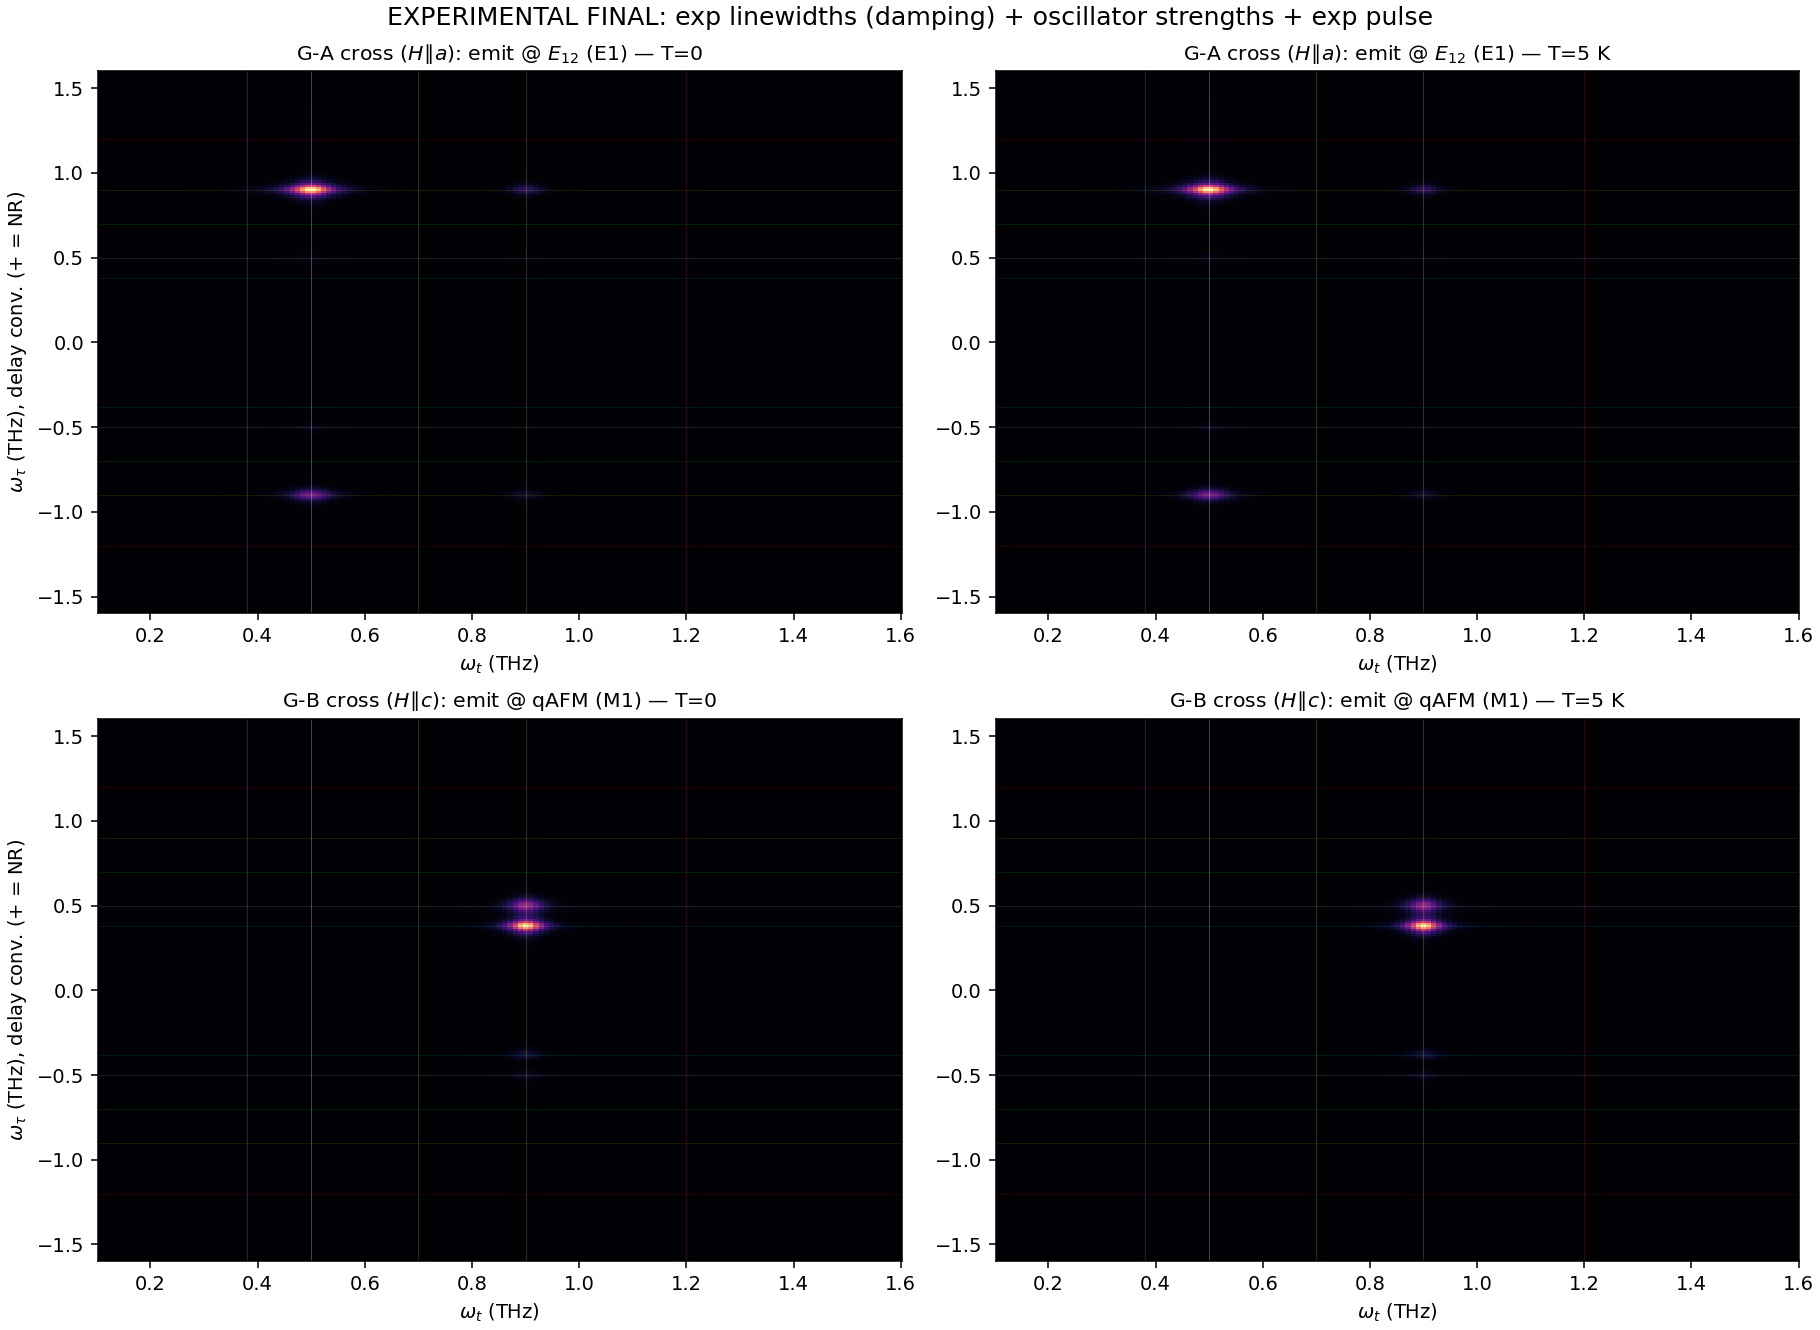
\includegraphics[width=\columnwidth]{../tmfeo3_2dcs_final/figures/crosspol_experimental_final.png}
\caption{Cross-polarized channels computed from experimental inputs
(measured pulse, linewidth damping, oscillator-strength emission).
Top: geometry A ($H\!\parallel\!a$), Tm $\lambda^2$ channel emitting at
$E_{12}$; the magnetoelectric $(\qafm,E_{12})$ cross peak dominates
(rephasing partner $0.33$).  Bottom: geometry B ($H\!\parallel\!c$),
magnon M1 channel emitting at $\qafm$; the magnon--magnon
$(\qfm,\qafm)$ and gated transfer $(E_{12},\qafm)$ peaks.  Left $T=0$,
right $T=5$\,K.}
\label{fig:crosspol}
\end{figure}

\emph{Geometry A, cross-polarized: a magnon read out through a CEF
dipole.}---During $\tau$ the Zeeman-launched $\qafm$ magnon precesses;
the static vertex $W^{yy}_1$, by which the magnon distortion modulates
the CEF splitting, transcribes the magnon phase onto the bright
$E_{12}$ coordinate.  The two-pulse cross term of $S_y^2$ rectifies,
\begin{equation}
  \Mnl^{W}\propto W^{yy}_1A^2\cos(\qafm\tau)\,[1-\cos E_{12}t],
  \label{eq:W}
\end{equation}
a factorized, rank-1 cross peak at $(\qafm,E_{12})$
[Fig.~\ref{fig:crosspol}, top].  The $E_{12}$ quantum is supplied by the
pulse-edge bandwidth (an intra-pulse difference-frequency process):
stretching the pulse from $\sigma=0.25$ to $1.0$ at fixed amplitude
collapses the peak by $4.5$ decades, the adiabatic suppression this
displacive mechanism demands, while switching off the direct Tm drive
changes it by $<10^{-4}$ [SI, Sec.~S6].  The peak is a
\emph{magnetoelectric} object: the E1-dark magnon borrows the Tm E1
dipole and emits at $E_{12}$, not at its own frequency.

\emph{Geometry B, cross-polarized: M1 readout and the two-vertex
division of labor.}---For $H\!\parallel\!c$ both observed peaks emit at
$\qafm$ through the magnon M1 dipole.  The magnon--magnon peak
$(\qfm,\qafm)$ requires no Fe--Tm physics (anisotropy plus DM couple the
branches).  The transfer peak $(E_{12},\qafm)$ isolates the second
vertex: with $\kappa^B_{1y}$ alone it is present ($0.46$); with the
static hybridization alone it is absent.  The field gate acts only while
$B_z(t)\neq0$, imprinting the stored $E_{12}$ phase impulsively on the
magnon---and the same gate makes $\kappa^B$ \emph{silent} in geometry A
($B_z=0$), where its background would otherwise contaminate the clean
$W$ peak.  Conversely, the measured post-drive buildup of the geometry-B
signal is impossible for a gated vertex and requires the static
$W^{xz}_1$ hybridization, whose slow exchange keeps pumping the magnon
after the field is gone [SI, Sec.~S7].  Neither vertex alone survives
the data; together they reproduce
$(\qfm,\qafm)=1.00$, $(E_{12},\qafm)=0.43$, residuals $\leq0.12$
[Fig.~\ref{fig:crosspol}, bottom].  The Tm CEF channels are identically
zero here: the $E\!\parallel\!a$, $H\!\parallel\!c$ drive closes on the
$\{\lambda^{1,2,3}\}$ subalgebra.

\begin{figure*}[t]

\includegraphics[width=\textwidth]{../tmfeo3_2dcs_final/figures/samepol_darkmu13_final.png}
\caption{Same-polarized geometry-A channel (blind census at $0$, $10$,
$20$\,K; crosses mark genuine local maxima).  Both transfer peaks,
$(+E_{12},E_{23})$ and $(+E_{12},E_{13})$, are non-rephasing, with the
$E_{23}$ member dominant; the rephasing remnant at $(-E_{12},E_{23})$
and the two-quantum line at $\omega_\tau=2E_{12}$ are predictions.
Right: the rectified signal $S_{\rm DC}(\tau)$ whose sharp line at
$+E_{12}$ is the $(E_{12},0)$ peak.}
\label{fig:samepol}
\end{figure*}

\emph{Geometry A, same-polarized: a dark dipole fixes the
hierarchy.}---The same-polarization channel ($E\!\parallel\!c$ in and
out) shows five features, in order
$(E_{12},E_{23})\approx(E_{12},0)>(E_{12},E_{13})>(\qafm,0.38),
(\qafm,E_{13})$, with \emph{both} CEF transfer peaks on the
non-rephasing side.  This inventory contains a structural clue: there is
no peak with delay phase $E_{13}=1.2$\,THz anywhere in the map.  A
bright $1\!\to\!3$ dipole would necessarily store an $E_{13}$ delay
coherence at first order and produce an $(E_{13},E_{23})$ peak with
\emph{exactly} the same dipole product $\mu_{12}\mu_{13}\mu_{23}$ as the
observed $(E_{12},E_{23})$ peak---no parameter choice can separate them.
The absence of the whole row is therefore a selection rule,
\begin{equation}
  \mu^{z}_{13}\simeq0,
  \label{eq:dark}
\end{equation}
the natural consequence of a parity-alternating CEF ladder
($\ket1,\ket3$ even, $\ket2$ odd under the site mirror): the
$z$-dipole connects $1\!\leftrightarrow\!2$ and $2\!\leftrightarrow\!3$
only.  The measured $E_{13}$ oscillator strength ($f=8.7$) lives in the
orthogonal polarizations---the same transition is bright in one
polarization and dark in the other.

Equation~\eqref{eq:dark} fixes three observables at once
[Fig.~\ref{fig:samepol}].  (i)~With the single-action (rephasing)
conversion route $\rho_{12}\!\to\!\rho_{32}$ removed, the dominant
transfer runs coherence$\to$population$\to$coherence: one probe action
converts the stored $E_{12}$ coherence into a level-2 population still
carrying the delay phase, a second converts it into the emitting
$E_{23}$ coherence.  This route is co-rotating and lands
\emph{non-rephasing}, the observed side; taken at its zero-frequency
output it also produces the $(E_{12},0)$ peak, a sharp $E_{12}$ line in
the rectified signal $S_{\rm DC}(\tau)$.  (ii)~The partner
$(E_{12},E_{13})$, though lower order, emits through the throttled
$\mu^z_{13}$ and is capped at $0.78$ of the dominant peak (the measured
ratio calibrates the residual admixture at the percent level).
(iii)~The magnon-delay peak $(\qafm,E_{13})$ is weak and thermally
activated ($0.10\to0.51$ from $0$ to $20$\,K).  The one feature the
model does not produce is $(\qafm,0.38)$: the $\qfm$ emission exists (a
$b$-axis M1 ridge, as $\Gamma_2$ symmetry requires) but no
$\qafm\!\to\!\qfm$ transfer vertex of sufficient strength exists in the
present Hamiltonian class [SI, Sec.~S8].

Because the single-ion dynamics is quantum-exact, these statements were
verified against a standalone qutrit integrator with the same pulse and
dampings, which reproduces the lattice census exactly and shows two
robust residuals that we advance as predictions: a rephasing remnant at
$(-E_{12},E_{23})$ at $\sim\!0.5$ of the dominant peak (an exact
single-ion floor under this pulse), and a lattice two-quantum line at
$\omega_\tau=2E_{12}=0.99$\,THz (absent in the single-ion dynamics,
i.e.\ a mean-field/inter-site product) [SI, Sec.~S8].

\emph{Predictions.}---Each mechanism carries its own falsifiable
signature.
(1)~\emph{Emission fingerprint}: the geometry-A cross peak emits at a
CEF frequency, the geometry-B peaks at the magnon frequency; any peak
emitting at $\qafm$ inherits the $15\times$ sharper magnon linewidth
along $\omega_t$.
(2)~\emph{Thermal trends}: $(\qfm,\qafm)$ is temperature-flat;
$(E_{12},\qafm)$ falls as the population difference $n_1-n_2$;
$(\qafm,E_{13})$ grows steeply; the same-polarization pair approaches
parity by $\sim20$\,K.
(3)~\emph{Polarization test of the dark dipole}: rotating either
polarization away from $c$ must revive the $\omega_\tau=1.2$\,THz delay
rows.
(4)~\emph{Field scaling}: the dominant $(E_{12},E_{23})$ peak is one
field order above $(E_{12},E_{13})$; lowering the fluence inverts their
order.
(5)~\emph{Sub-features}: the rephasing remnant at $(-E_{12},E_{23})$
and the two-quantum line at $\omega_\tau=0.99$\,THz (resolvable from the
$0.90$ magnon row) should both be present in raw data.
(6)~\emph{Pulse-length test}: the geometry-A cross peak is displacive
and collapses for adiabatically long pulses.

\emph{Conclusion.}---A single Fe--Tm Hamiltonian with two
symmetry-selected vertices, driven by the measured pulse and dressed
with measured linewidths and oscillator strengths, accounts for the
complete 2DCS peak inventory of TmFeO$_3$ across three detection
channels.  The analysis illustrates a general program for
magnon--crystal-field 2DCS: time-reversal and irrep bookkeeping reduce
the coupling space to a few vertices; emission dipoles (E1 versus M1)
decide where each coherence is read out; and polarization-resolved
selection rules---here a $z$-dark $1\!\to\!3$ dipole---control the
pathway orders and hence the signed-side structure of the 2D map.
The framework, and the quantum-exactness of the SU(3) single-ion
dynamics, carry over directly to other rare-earth orthoferrites and to
singlet-ladder magnets generally.

\begin{acknowledgments}
Numerical details, derivations, and the complete falsification ledger
are given in the Supplemental Material.
\end{acknowledgments}

\bibliographystyle{apsrev4-2}
\begin{thebibliography}{9}
\bibitem{Lu2017} J. Lu, X. Li, H. Y. Hwang, B. K. Ofori-Okai,
  T. Kurihara, T. Suemoto, and K. A. Nelson,
  Phys.\ Rev.\ Lett.\ \textbf{118}, 207204 (2017).
\bibitem{Mukamel} S. Mukamel, \emph{Principles of Nonlinear Optical
  Spectroscopy} (Oxford University Press, New York, 1995).
\bibitem{Yamaguchi} T. Yamaguchi,
  J.\ Phys.\ Chem.\ Solids \textbf{35}, 479 (1974).
\bibitem{Kimel2004} A. V. Kimel, A. Kirilyuk, A. Tsvetkov, R. V.
  Pisarev, and Th. Rasing, Nature \textbf{429}, 850 (2004).
\bibitem{Zhang2016} \emph{Resolving the spin reorientation and
  crystal-field transitions in TmFeO$_3$ with terahertz transient},
  Sci.\ Rep.\ \textbf{6}, 23648 (2016).
\bibitem{MP2018} \emph{Terahertz magnon-polaritons in TmFeO$_3$},
  ACS Photonics \textbf{5}, 1375 (2018).
\end{thebibliography}

\end{document}
